
	
\chapter{Implementacija i korisničko sučelje}
		
		
		\section{Korištene tehnologije i alati}

		Komunikacija našem u timu je realizirana korištenjem aplikacija Discord\footnote{https://discord.com/} i WhatsApp\footnote{https://www.whatsapp.com/}.\\ Za izradu UML dijagrama korišten je alat Astah Professional\footnote{http://astah.net/editions/professional}, a kao sustav za upravljanje
izvornim kodom Git\footnote{https://git-scm.com/}. Udaljeni repozitorij projekta je dostupan na web platformi GitLab\footnote{https://gitlab.com/}, a kao razvojno okruženje korišten je IntelliJ IDEA\footnote{https://www.jetbrains.com/idea/} - tvrtke JetBrains\footnote{https://www.jetbrains.com/} te Microsoftov Visual Studio Code\footnote{https://visualstudio.microsoft.com/
}. 
	\\
	 Naša aplikacija napisana je koristeći Spring Framework\footnote{https://spring.io/} i jezik Java\footnote{https://www.oracle.com/java/} za izradu backenda te React\footnote{https://reactjs.org/} - JavaScript library za izradu frontenda. React je open-source, front end, JavaScript knjižnica za izgradnju korisničkog sučelja ili UI komponenti. Održavaju ga Facebook i zajednica pojedinačnih programera i tvrtki. Spring razvojno okruženje je Java platforma koja pruža široki panel opcija kao podrški
razvoju Java aplikacija. Spring rukuje infrastrukturom, tako da programer može usmjeriti svoj
fokus na razvoj aplikacije. \\
Tijekom izrađivanja aplikacije koristili smo i Postman\footnote{https://www.postman.com/} za simuliranje HTTP zahtjeva nad aplikacijom, Google Drive\footnote{https://workspace.google.com/products/drive/} za efikasno dijeljenje organizacijskih informacija i raznih datoteka. 
Baza podataka se nalazi na poslužitelju u oblaku Amazon
Web Services\footnote{https://aws.amazon.com/}.			
			
			\eject 
		
	
		\section{Ispitivanje programskog rješenja}

	
			
			\subsection{Ispitivanje komponenti}

			\textbf{Unit testovi za Service sloj}
			\bigskip
			\newline
			Za izradu unit testova korišten je framework Mockito, koji simulira rad objekata koje testni razred koristi.  
			 @Mock anotacija stvara objekt koji se koristi u testiranju, on ne izvodi svoje normalne metode, već samo simulira njihov rad.
			\bigskip
			\bigskip
			
			\bigskip
			\textbf{UserServiceJpa unit test}
			\bigskip
			
			\textit{listAll()} - U unit testu stvaramo 3 nova korisnika i simuliramo metodu listAll(). Očekivani rezultat je lista tri korisnika. Zatim pozovemo metodu listAll() i provjerimo vraća li ta metoda ispravni izlaz.
			
			\textit{registerUser()} - Unit testovi za ovu metodu ispituju ponašanje sustava za neuspješnu i uspješnu registraciju.
			
			\textit{updateUser()} - Testovi ispituju ponašanje sustava prilikom pokušaja ažuriranja korisničkih podataka. Pokriveni su slučajevi potpunih i nepotpunih podataka za ažuriranje.
			
			\textit{findByUsername()} - Testovi ispituju ponašanje sustava pri pretraživanju korisnika za postojeće i nepostojeće korisničko ime.
			
			\textit{getStatistics()} - Ukoliko ne postoje registrirani korisnici pri pozivu ove metode, ona bi trebala vratiti praznu listu. Ako postoje registrirani korisnici, ali ne njih više od dva, metoda bi trebala vratiti samo listu od tog jednog ili dva korisnika, tako da je prvi onaj bolje ocjenjeni. Ako postoji tri ili više registriranih korisnika metoda bi trebala vratiti listu od tri najbolje ocjenjena korisnika. Testira se i u kojem poretku je metoda vratila najbolje ocijenjene korisnike.
			
			\bigskip
			\bigskip
			\textbf{RatingServiceJpa unit test}
			\bigskip
			
			\textit{calculateAverageRatingForUser()} - Metoda ispituje  izračun prosječne ocjene za korisnika. Ulaz je korisničko ime, a izlaz ovisi o postojanju korisnika s danim korisničkim imenom i postojanju ocjena.
			
			\bigskip
			\bigskip
			\textbf{RequestServiceJpa unit test}
			\bigskip
			
			\textit{addRequest()} - Metoda testira potpunost podataka prilikom stvaranja zahtjeva. Ako je predan zahtjev koji je potpun i točan metoda bi trebala uspješno dodati zahtjev. U suprotnom metoda testira odgovarajuće iznimke.
			
			\bigskip
			\begin{figure}[H]
				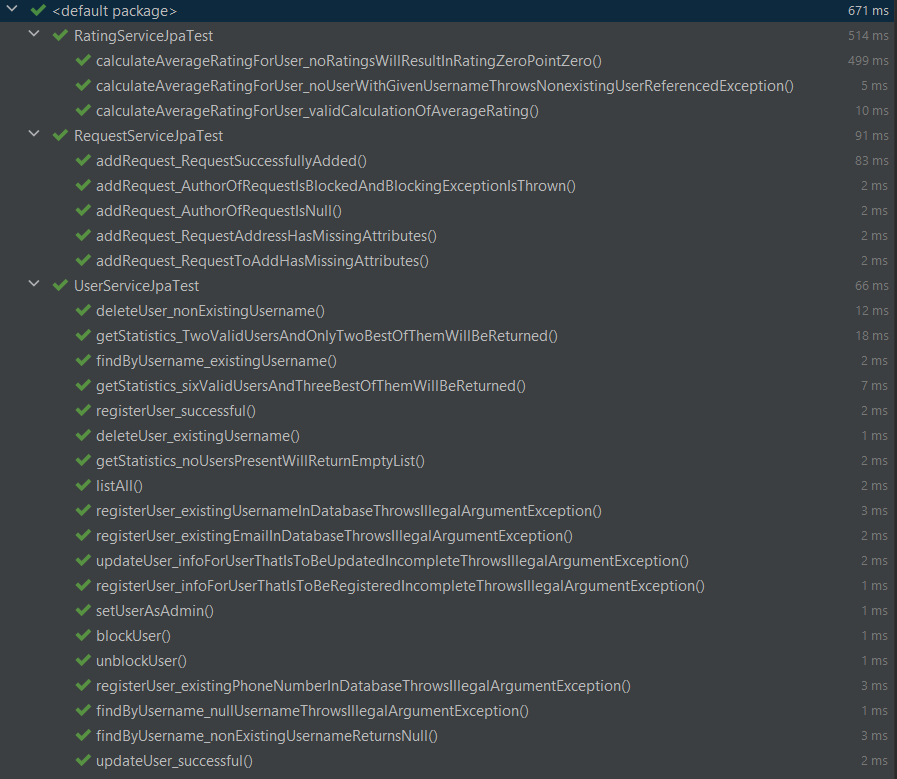
\includegraphics[scale=0.8]{slike/unit_testovi.png}
				\centering
				\caption{Rezultati unit testova}
				
			\end{figure}
			
			
			\subsection{Ispitivanje sustava}
			
			Za ispitivanje sustava korišten je alat za automatizirano testiranje Selenium WebDriver. Ispitni slučajevi pisani
			su u jeziku Java. \newline
			
			Cilj ispitivanja sustava je ispitati ponašanje sustava u cjelini, onako kako ga vidi 
			korisnik aplikacije te dostupnost svih funkcionalnosti koje korisnik može koristiti.
			Napisani ispitni slučajevi prije svega su ispitivali pravilan izgled komponenti i funkcionalnosti koje se nude kroz korisničko sučelje u ovisnosti o stanju sustava, stanju pojedinog zahtjeva i ovlastima korisnika.
			Testiranje je koristilo dva korisnika već registrirana u sustav, jednog s ovlastima običnog korisnika i drugog s ovlastima administratora.\newline 
			
			Komponente koje najviše ovise o ovlastima i stanju sustava su komponenta za prikaz pojedinog zahtjeva i komponenta profila korisnika.
			Za primjer, funkcionalnosti rada sa zahtjevima testiraju metode:
			\begin{packed_enum}
				
				\item \textit{createRequestExpectedBehaviour()} - očekivani unos u formu zahtjeva
				\item \textit{createRequestNoTitle()} - neispravan unos u formu zahtjeva
				\item \textit{viewNonAuthoredRequest()} - prisutnost komponenti za javljanje na zahtjev
				\item \textit{viewAuthoredRequest()} - prisutnost komponenti za blokiranje zahtjeva
				\item \textit{viewAuthoredRequestWithPotentialHandlers()} - prisutnost komponenti za pregled potencijalnih izvršitelja 
			\end{packed_enum}
			
		
			
			Testni slučajevi fokusirali su se na različite situacije i rubne slučajeve u prikazu i funkcionalnostima.
			Rubni slučajevi poput pogrešnog unosa u formu ili nedostatka nekog unosa se u aplikaciji signaliziraju različitim porukama o pogrešci. 
			Testne metode za takve slučajeve prije svega su se fokusirali na traženje odgovarajuće poruke o pogrešci.
			Konkretan primjer za to su testni slučajevi unosa pogrešnih korisničkih podataka u formu za prijavu. \newline 
			
			Neimplementirana funkcionalnost koja je također testirana je traka za pretraživanje. 
			Testom je pokazano da akcijama nad njom se ne mjenja stanje sustava i ne remeti se normalan tijek funkcioniranja aplikacije. \newline
			
			Glavnu prepreku za automatizaciju ispitivanja sustava predstavljala je priroda testiranog sustava. 
			Sustav se sastoji od brojnih aktivnosti koje se mogu izvoditi samo jednom, poput javljanja na pojedini zahtjev ili 
			biranja izvršitelja za zahtjev te aktivnosti koje zahtijevaju slijednu interakciju više korisnika.
			Takve akcije teško je automatizirano ispitivati zato što to neminovno u sustavu akumulira velik broj zahtjeva samo za testiranje 
			ili testove nije moguće ponavljati više puta, čime se u potpunosti gubi njihova svrha.
			Stoga su navedene funkcionalnosti izostavljene iz automatiziranog ispitvanja alatom Selenium i odrađene ručno.
			
			
			
			
			\begin{figure}[H]
				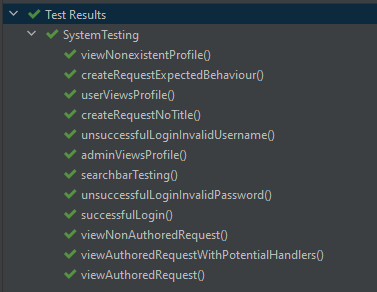
\includegraphics[scale=1.2]{slike/selenium-testing.png}
				\centering
				\caption{Rezultati testova sustava}
				
			\end{figure}
			
			 
			
			\eject 
		
		
		\section{Dijagram razmještaja}
			
			Na slici 5.3 nalazi se dijagram razmještaja koji prikazuje raspored programske podrške aplikaciji unutar sklopovlja.
			
			Sa strane korisnika aplikacije, sklopovlje predstavlja njegovo računalo, mobilni telefon ili bilo koji drugi uređaj s pristupom internetu i instaliranim browserom.
			Internetski browser zadužen je za uspostavu konekcije sa poslužiteljem koja će omogućiti slanje i posluživanje zahtjeva.
			Sa strane poslužitelja sklopovlje predstavlja serversko računalo.
			Dvije glavne usluge koje se nalaze na serverskom računalu su baza podataka i web server koje su nužne za posluživanje zahtjeva.
			
			Komunikacija između korisnika i poslužitelja vrši se putem \textit{stateless} HTTP protokola. 
			Tijekom slanja zahtjeva serveru, korisnikov browser ima otvorenu jednu HTTP vezu prema serveru.
			S druge strane server može posluživati više zahtjeva iz više različitih izvora te stoga može imati i više aktivnih HTTP veza.
			
			\begin{figure}[h]
				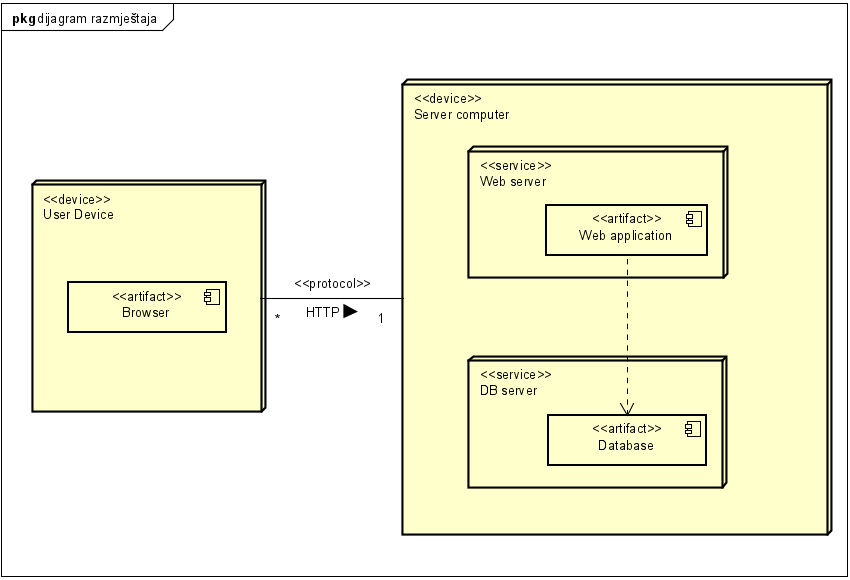
\includegraphics[height=0.44\textheight]{dijagramRazmjestaja}
				\caption{Dijagram razmještaja}
			\end{figure} 
			
			\eject 
		
		\section{Upute za puštanje u pogon}
		
			Grupa TODO odlučila je aplikaciju pustiti u pogon koristeći Amazon Web Services (AWS). Za korištenje AWS-a potrebno se registrirati i ostaviti podatke za plaćanje, ali koriste se besplatne mogućnosti dostupnih usluga te ništa neće biti naplaćeno. 
			
			Korisnik nakon registracije, odlazi na adresu \url{https://us-east-2.console.aws.amazon.com/console/home}, gdje dobiva prikaz dostupnih usluga:
			
			\begin{figure}[h]
				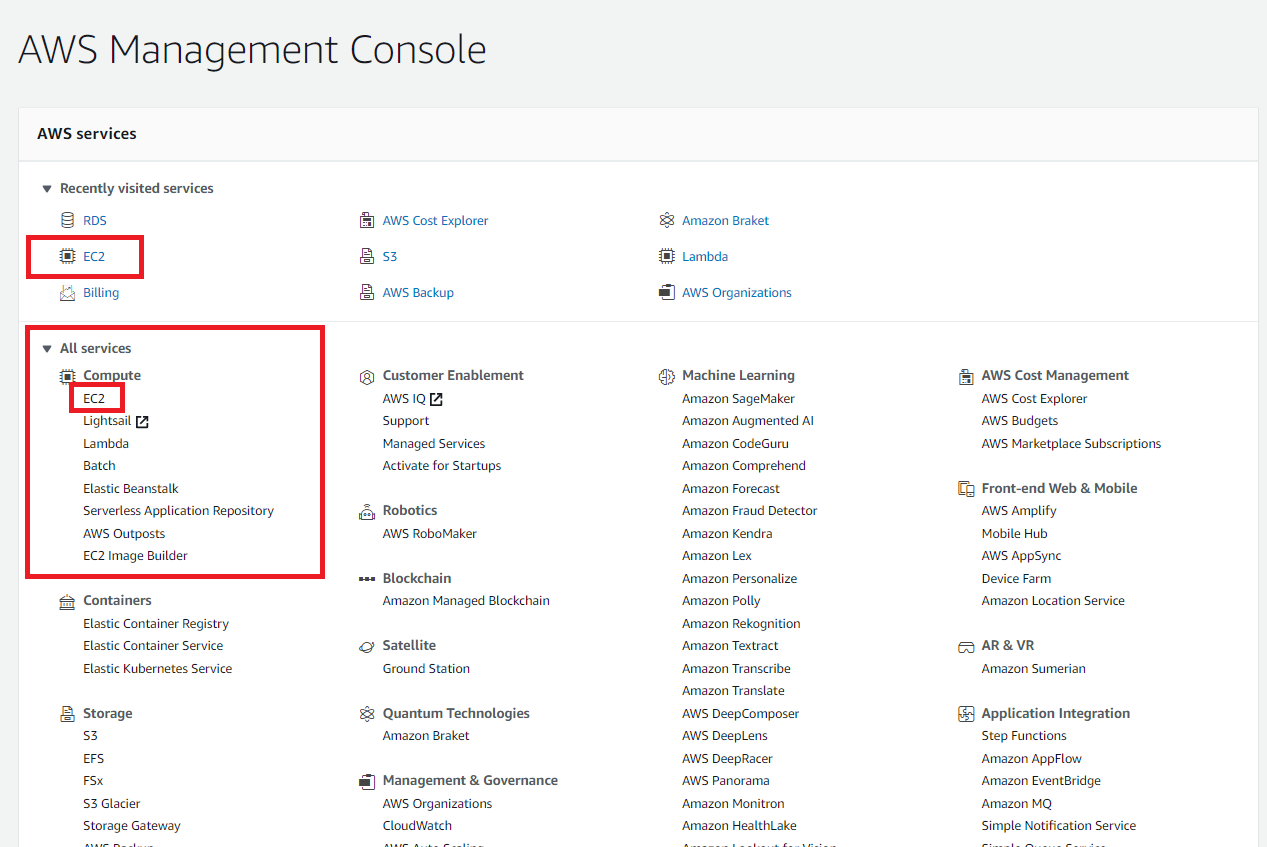
\includegraphics[scale=0.5]{slike/deployment_slike/awshome.png}
				\centering
				\caption{Dostupne AWS usluge}
				
			\end{figure}
		
			Biramo link EC2  koji nas vodi na iduću stranicu,gdje želimo stisnuti na pokretanje nove instance virtualnog stroja (Slika 5.4), potom odabiremo operacijski sustav virtualnog stroja(Slika 5.5). Biramo OS sa slike zato što je dostupan za besplatno korištenje. U idućem koraku ponovo odabiremo besplatan tip instance (Slika 5.6), klikamo Review and Launch i Launch, postavljamo i preuzimamo ključ za pristup instanci (neće biti potreban, al ga je dobro pričuvat). Posljednji put pritišćemo Launch i pokreće se instanciranje virtualnog stroja. Zatim na adresi \url{https://us-east-2.console.aws.amazon.com/ec2/v2/home} možemo pregledati vlastite instance virtualnih strojeva (Slika 5.7). Na "running" instancu desni klik i Connect. Možemo birati više načina spajanja, biramo treću opciju zbog jednostavnosti i pritišćemo gumb Connect (Slika 5.8). Otvara nam se linux terminal u browseru (Slika 5.9) i možemo krenuti s konfiguracijom virtualnog stroja.
			
			
			\noindent Prvo unosimo naredbu:
			\begin{center}
				\$ sudo yum update
			\end{center}
				kako bi primjenili ažuriranja. Za uspješno puštanje u pogon potrebni su nam Java, Git i Maven. Njih ćemo instalirati redom upisujući naredbe
				\begin{center}
					\$ sudo yum install java-11
				\end{center}
			\begin{center}
				\$ sudo yum alternatives  \texttt{--}config java
			\end{center}
			otvara nam se izbornik te odabiremo željenu verziju jave (Java 11 Amazon Corretto) unosom rednog broja pored imena verzije.
			Maven instaliravamo sljedećim nizom naredbi:
			\begin{center}
				\$ sudo wget http://repos.fedorapeople.org/repos/dchen/apache-maven/epel-apache-maven.repo -O /etc/yum.repos.d/epel-apache-maven.repo
				
				\$ sudo sed -i s/$\backslash$\$releasever/6/g /etc/yum.repos.d/epel-apache-maven.repo
				
				\$ sudo yum install -y apache-maven
			
				\$ mvn --version
			\end{center}
			Dalje, unosimo naredbe:
			\begin{center}
				\$ sudo yum install git -y
				
				\$ git clone \{adresa repozitorija\}
			\end{center}
			Nakon toga potrebno se pozicionirati u direktorij izvornog koda (onaj gdje se nalazi pom.xml), i pokrenuti instalaciju naredbom:
			\begin{center}
				\$ mvn clean install
			\end{center}
			Nakon instalacije, u direktoriju /target nalazi se .jar datoteka koja predstavlja našu izgrađenu aplikaciju. Aplikaciju pokrećemo izvođenjem sljedeće naredbe:
			\begin{center}
				\$ nohup java -jar \{ime aplikacije\}.jar
			\end{center}
			Aplikacija je nakon nekoliko trenutaka pokrenuta i moguće joj je pristupiti preko javne adrese instance, na portu 8080, ali tek nakon što u AWS konzoli podesimo parametre sigurnosti, upute za to ostavljamo da korisnik sam prouči: \url{https://docs.aws.amazon.com/AWSEC2/latest/UserGuide/ec2-security-groups.html}
		
		
		
			
			\begin{figure}[h]
				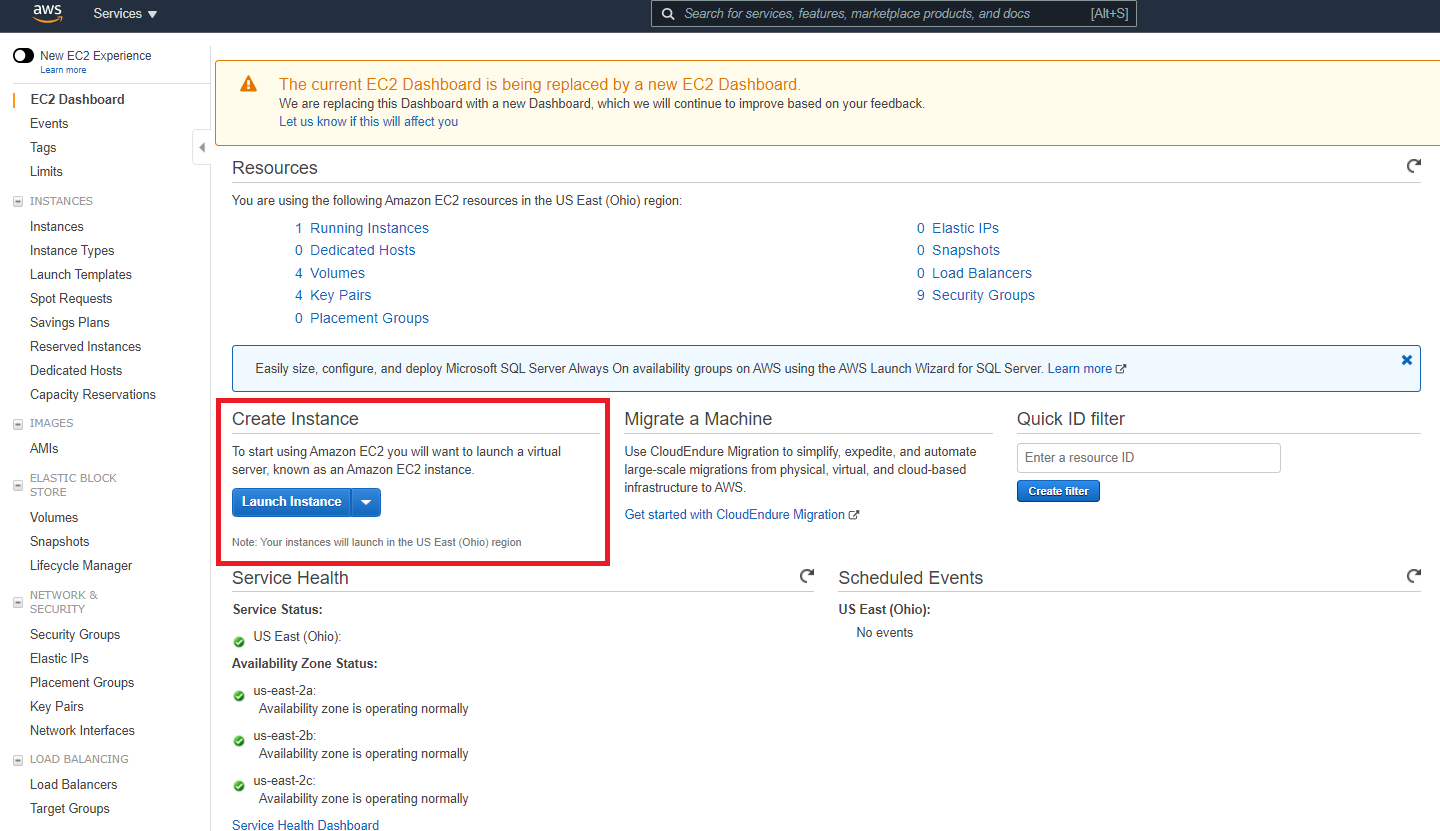
\includegraphics[width=\textwidth]{slike/deployment_slike/launchingInstance.png}
				\centering
				\caption{Pokretanje inicijalizacije}
			\end{figure}
		
			\begin{figure}[h]
				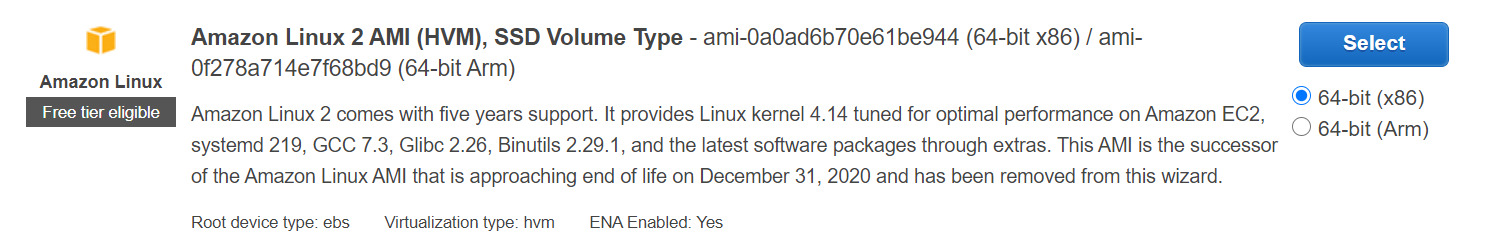
\includegraphics[width=\textwidth]{slike/deployment_slike/virtualOS.png}
				\centering
				\caption{Odabrani OS}
			\end{figure}
		
			\begin{figure}[h]
				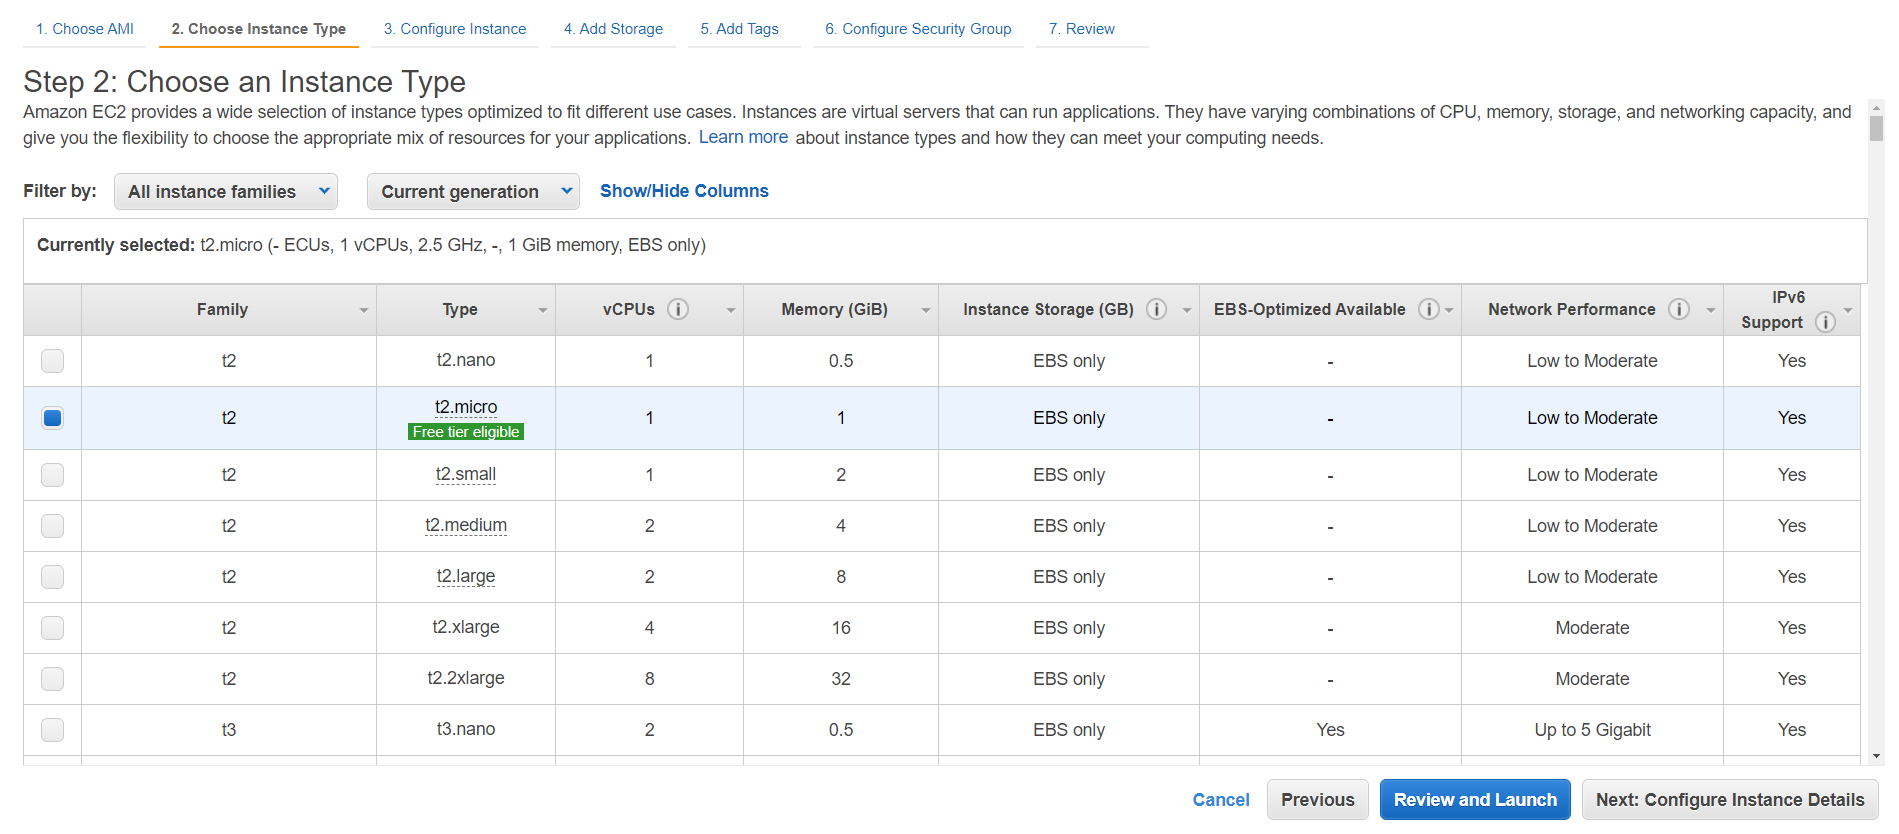
\includegraphics[width=\textwidth]{slike/deployment_slike/instanceType.png}
				\centering
				\caption{Tip instance}
			\end{figure}
			
			\begin{figure}[h]
				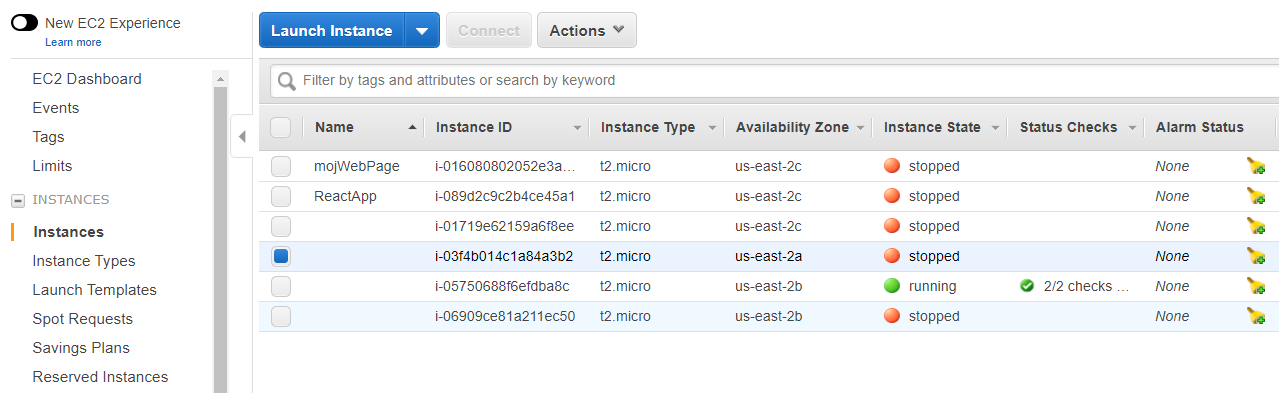
\includegraphics[width=\textwidth]{slike/deployment_slike/mojeInstance.png}
				\centering
				\caption{Instance}
			\end{figure}
			
			\begin{figure}[h]
				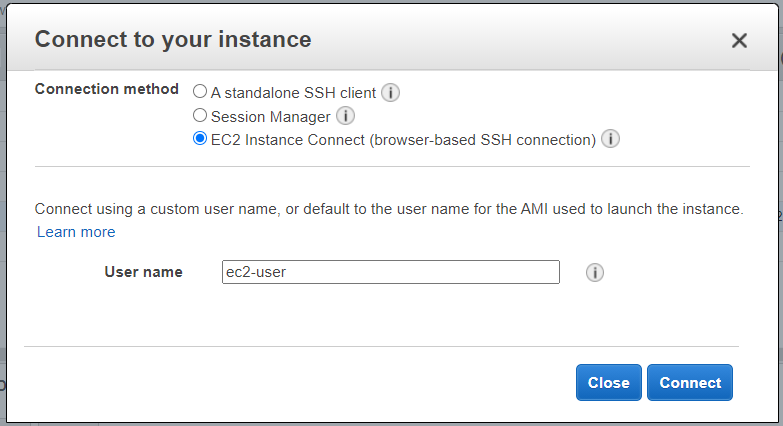
\includegraphics[width=\textwidth]{slike/deployment_slike/instanceConnect.png}
				\centering
				\caption{Spajanje na virtualni stroj}
			\end{figure}
		
			\begin{figure}[h]
				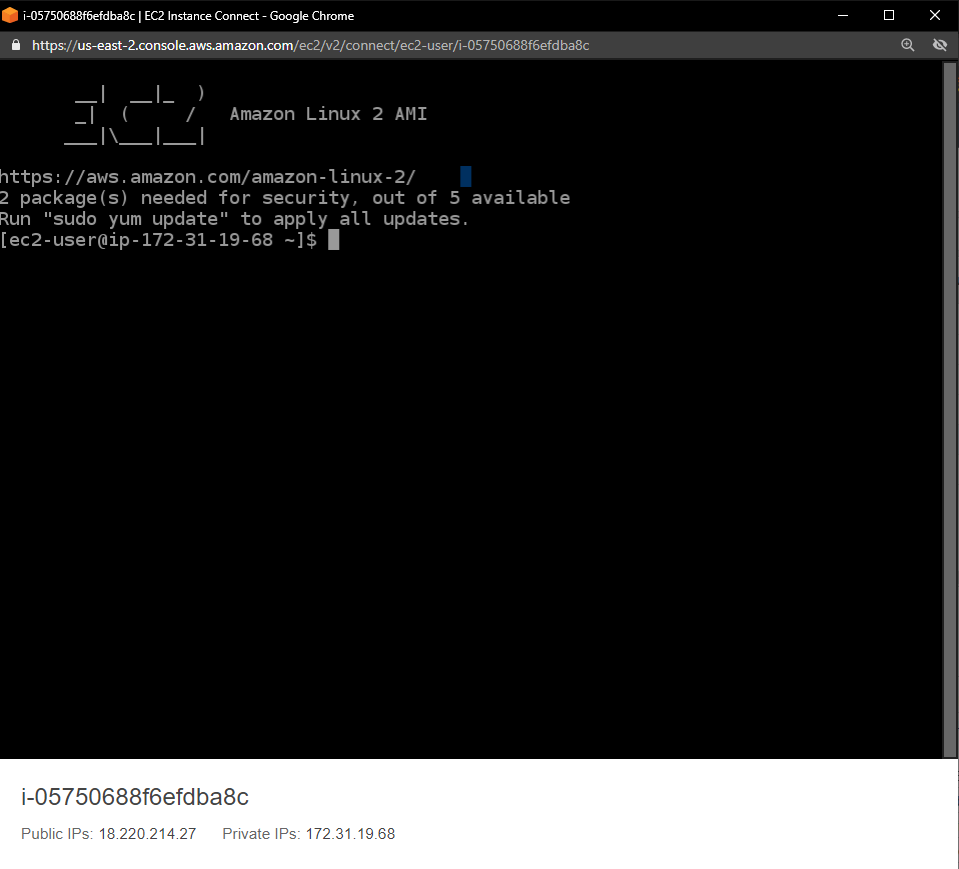
\includegraphics[width=\textwidth]{slike/deployment_slike/browserTerminal.png}
				\centering
				\caption{Browser terminal}
			\end{figure}
			
			\eject 